Solve the analogous problem in 3D, that is, given a 3D point cloud, find an implicit surface that approximates the point
cloud surface via RBF interpolation.

\begin{solution}
  We now consider the 3D version of the Fernandez-Guasti equation

  $$
  x^2 + y^2 + z^2 - s^2 \left(x^2 y^2 + y^2 z^2 + x^2 z^2 \right) + s^4 x^2 y^2 z^2 = 1
  $$

  with squareness parameter $s$. When $s = 0$, the above equation represents a sphere of radius 1; when $s = 1$, the 
  equation corresponds to a cube of side length 2. When $0 < s < 1$, the resulting shape is somewhere in between the 
  two. With a squelched sphere-to-cube mapping (from the same source as in Problem 1), this becomes the system of 
  parametric equations:

  $$
  f(x, y, z) = \begin{cases}
    x(\theta, \phi) = \frac{\cos{\theta} \cos{\phi}}{\sqrt{1 - s \cos^2{\theta} \sin^2{\phi} - s \sin^2{\theta}}} \\
    y(\theta, \phi) = \frac{\cos{\theta} \sin{\phi}}{\sqrt{1 - s \cos^2{\theta} \cos^2{\phi} - s \sin^2{\theta}}} \\
    z(\theta, \phi) = \frac{\sin{\theta}}{\sqrt{1 - s \cos^2{\theta}}}
  \end{cases}, \quad \theta, \phi \in [0, 2 \pi]
  $$

  We generate the point cloud in Figure \ref{fig:problem_2ii_source_cloud} with $s=0.75$ and random noise in the $x$ 
  direction in \texttt{problem\_2ii.m}. 
 
  \begin{figure}[h]
    \centering
    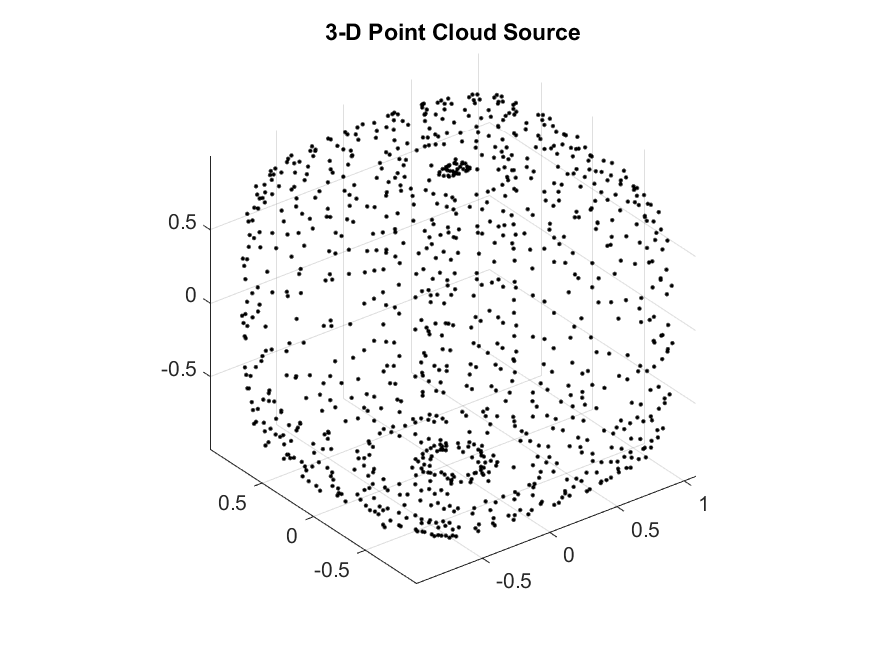
\includegraphics[width=.9\textwidth]{problem_2ii_source_cloud.png}
    \caption{Source point cloud}
    \label{fig:problem_2ii_source_cloud}
  \end{figure}
 
  \pagebreak
  We then compute normal directions $\bm{n}_j$ at each point to obtain $\bm{x}^-_j$ and $\bm{x}^+_j$ and perform RBF
  interpolation as in Problem 2i. We obtain Figure \ref{fig:problem_2ii_rbf_interpolant} upon projecting the resulting 
  interpolant $F(\alpha)$ to the isosurface $\alpha = 0$.

  \begin{figure}[h]
    \centering
    \begin{subfigure}{\textwidth}
        \centering
        \includegraphics*[width=.625\textwidth]{problem_2ii_normal_cloud_2d.png}
        \caption{2D projection of source point cloud and normal directions}
        \label{fig:problem_2ii_normal_cloud_2d}
    \end{subfigure}
    \begin{subfigure}{\textwidth}
        \centering
        \includegraphics*[width=.625\textwidth]{problem_2ii_rbf_surface.png}
        \caption{3D RBF Interpolant}
        \label{fig:problem_2ii_rbf_surface}
    \end{subfigure}
    \caption{Japanese watermelon interpolation}
    \label{fig:problem_2ii_rbf_interpolant}
  \end{figure}
\end{solution}